\documentclass[tikz,border=8pt]{standalone}
\usepackage{amsmath}
% Shared UMM figure style (journal-consistent palette + line weights)
\usepackage{tikz}
\usepackage{pgfplots}
\pgfplotsset{compat=1.18}
\usetikzlibrary{arrows.meta,calc,positioning,decorations.pathmorphing,patterns,shapes.geometric,fit,backgrounds}
% Palette: grayscale + single accent (deep teal)
\definecolor{ummAccent}{HTML}{0B6E6E}
\definecolor{ummAccentLight}{HTML}{4A9B9B}
\definecolor{ummDark}{HTML}{1A1A1A}
\definecolor{ummGray}{HTML}{555555}
\definecolor{ummLightGray}{HTML}{AAAAAA}
\definecolor{ummFill}{HTML}{E8F2F2}
\definecolor{ummGas}{HTML}{C45C26}
\definecolor{ummGasLight}{HTML}{F0C4A8}
\definecolor{ummGalaxy}{HTML}{2C3E50}
\definecolor{ummLens}{HTML}{0B6E6E}
\pgfplotsset{
  umm axis/.style={
    axis lines=left,
    axis line style={ummDark, line width=0.8pt},
    tick style={ummDark, line width=0.6pt},
    tick label style={font=\footnotesize, ummDark},
    label style={font=\small, ummDark},
    title style={font=\small\bfseries, ummDark},
    grid=both,
    major grid style={ummLightGray, opacity=0.35, line width=0.3pt},
    minor grid style={ummLightGray, opacity=0.15, line width=0.2pt},
    every axis plot/.append style={line width=1.3pt},
    legend style={font=\footnotesize, draw=ummLightGray, fill=white, fill opacity=0.92, text opacity=1},
    clip=false,
  },
}
\newcommand{\ummLineW}{1.25pt}
\newcommand{\ummLineWthin}{0.9pt}
\tikzset{
  umm arr/.style={-{Latex[length=2.2mm,width=1.6mm]}},
}

\begin{document}
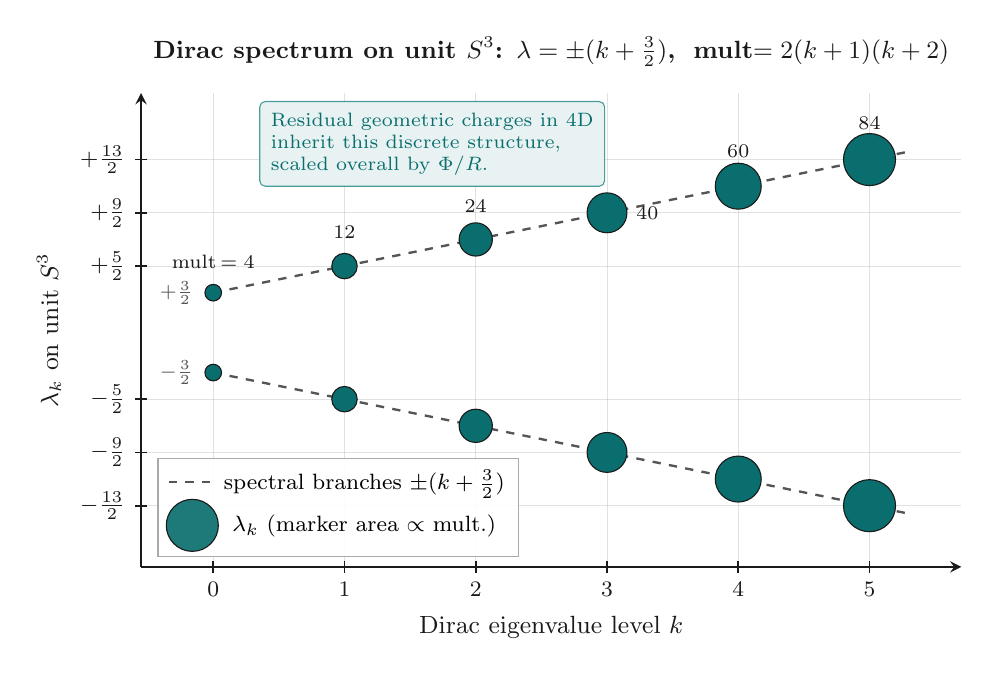
\begin{tikzpicture}
\begin{axis}[
  umm axis,
  width=12.0cm,
  height=7.6cm,
  xlabel={Dirac eigenvalue level $k$},
  ylabel={$\lambda_k$ on unit $S^3$},
  xmin=-0.55, xmax=5.7,
  ymin=-8.8, ymax=9.0,
  xtick={0,1,2,3,4,5},
  ytick={-6.5,-4.5,-2.5,2.5,4.5,6.5},
  yticklabels={$-\tfrac{13}{2}$,$-\tfrac{9}{2}$,$-\tfrac{5}{2}$,
               $+\tfrac{5}{2}$,$+\tfrac{9}{2}$,$+\tfrac{13}{2}$},
  legend style={at={(0.02,0.02)}, anchor=south west, font=\footnotesize},
  title={Dirac spectrum on unit $S^3$: $\lambda=\pm(k+\tfrac{3}{2})$,\; mult$=2(k+1)(k+2)$},
]
  % Guide lines lambda = ±(k+3/2)
  \addplot[ummGray, dashed, line width=0.85pt, domain=0:5.3, samples=2] {x+1.5};
  \addlegendentry{spectral branches $\pm(k+\tfrac{3}{2})$}
  \addplot[ummGray, dashed, line width=0.85pt, domain=0:5.3, samples=2, forget plot] {-x-1.5};

  % Eigenvalues; mark size scales with multiplicity
  \addplot[only marks, mark=*, ummAccent, draw=ummDark, line width=0.4pt,
           mark size=3.0pt, forget plot] coordinates {(0,1.5) (0,-1.5)};
  \addplot[only marks, mark=*, ummAccent, draw=ummDark, line width=0.4pt,
           mark size=4.6pt, forget plot] coordinates {(1,2.5) (1,-2.5)};
  \addplot[only marks, mark=*, ummAccent, draw=ummDark, line width=0.4pt,
           mark size=6.0pt, forget plot] coordinates {(2,3.5) (2,-3.5)};
  \addplot[only marks, mark=*, ummAccent, draw=ummDark, line width=0.4pt,
           mark size=7.2pt, forget plot] coordinates {(3,4.5) (3,-4.5)};
  \addplot[only marks, mark=*, ummAccent, draw=ummDark, line width=0.4pt,
           mark size=8.3pt, forget plot] coordinates {(4,5.5) (4,-5.5)};
  \addplot[only marks, mark=*, ummAccent, draw=ummDark, line width=0.4pt,
           mark size=9.4pt] coordinates {(5,6.5) (5,-6.5)};
  \addlegendentry{$\lambda_k$ (marker area $\propto$ mult.)}

  % Multiplicity annotations (positive branch only)
  \node[font=\scriptsize, ummDark, anchor=south] at (axis cs:0,2.05) {mult\,$=4$};
  \node[font=\scriptsize, ummDark, anchor=south] at (axis cs:1,3.15) {$12$};
  \node[font=\scriptsize, ummDark, anchor=south] at (axis cs:2,4.15) {$24$};
  \node[font=\scriptsize, ummDark, anchor=west] at (axis cs:3.15,4.5) {$40$};
  \node[font=\scriptsize, ummDark, anchor=south] at (axis cs:4,6.2) {$60$};
  \node[font=\scriptsize, ummDark, anchor=south] at (axis cs:5,7.25) {$84$};

  % Also label ±3/2 explicitly near lowest
  \node[font=\scriptsize, ummGray, anchor=east] at (axis cs:-0.08,1.5) {$+\tfrac{3}{2}$};
  \node[font=\scriptsize, ummGray, anchor=east] at (axis cs:-0.08,-1.5) {$-\tfrac{3}{2}$};

  % Phi scaling note (upper center-left, clear of large markers)
  \node[font=\scriptsize, ummAccent, align=left, anchor=north west,
        fill=ummFill, draw=ummAccentLight, inner sep=4pt, rounded corners=2pt]
    at (axis cs:0.35,8.7)
    {Residual geometric charges in 4D\\
     inherit this discrete structure,\\
     scaled overall by $\Phi/R$.};
\end{axis}
\end{tikzpicture}
\end{document}
